\documentclass[12pt]{article}
\usepackage{graphicx}
\usepackage{amsmath}
\usepackage{hyperref}
\usepackage{geometry}
\geometry{margin=1in}
\title{Python4Physics 2025 -- Final Report}
\author{Arnav Kapoor}
\date{}
\begin{document}
\maketitle
\noindent Email: \texttt{your.email@domain.com}

\section*{Introduction}
The Python4Physics 2025 program was an enriching experience that deepened my understanding of both physics and scientific computing. Over the course of the program, I engaged with a variety of topics, including data visualization, probability and statistics, Monte Carlo methods, and the simulation of physical systems. This report reflects on the key concepts I learned, projects I enjoyed, and insights gained from lectures and guest presentations.

\section*{Daily Highlights}
\begin{itemize}
  \item \textbf{Day 1: Introduction to Python and Plotting} -- Learned the basics of Python syntax and Jupyter notebooks. Explored data visualization with matplotlib, creating plots of mathematical functions and customizing their appearance.
  \item \textbf{Day 2: Arrays, Lists, and Data Structures} -- Gained experience with numpy arrays and Python lists, understanding their differences and use cases. Practiced manipulating arrays and performing vectorized operations for efficient computation.
  \item \textbf{Day 3: Probability and Random Numbers} -- Studied the generation of random numbers and their applications in simulations. Implemented Monte Carlo methods to estimate mathematical constants such as $\pi$.
  \item \textbf{Day 4: Statistics and Distributions} -- Learned about Gaussian (normal) distributions and how to generate and visualize them in Python. Used histograms to analyze the distribution of simulated data and compared it to theoretical curves.
  \item \textbf{Day 5: Data Handling and File I/O} -- Practiced saving and loading data using numpy's file I/O functions. Understood the importance of reproducibility and data management in scientific research.
  \item \textbf{Day 6: Advanced Plotting and Data Analysis} -- Created multi-panel plots and explored advanced features of matplotlib. Analyzed real and simulated datasets, extracting meaningful statistics and trends.
  \item \textbf{Day 7: Physics Simulations -- Projectile Motion} -- Modeled projectile motion using Python, varying initial conditions and visualizing trajectories. Connected physical principles with computational models to deepen understanding of kinematics.
  \item \textbf{Day 8: Project Work and Collaboration} -- Worked on a capstone project, applying skills learned throughout the program to a larger problem. Collaborated with peers, shared code, and presented findings to the group.
  \item \textbf{Day 9: Guest Lectures and Research Applications} -- Attended guest lectures on topics such as computational astrophysics and data science in physics. Learned how Python is used in cutting-edge research and discussed career pathways in computational science.
\end{itemize}

\section*{Summary of Lectures}
Each day's lectures built upon the previous, gradually increasing in complexity and depth. The combination of theory, hands-on coding, and real-world applications made the learning process engaging and effective. The guest speakers provided valuable insights into how the skills we developed are used in academic and industry research.

\section*{Key Learnings}
\begin{enumerate}
  \item \textbf{Scientific Computing with Python} -- Mastery of Python for scientific computing and data analysis, including numpy, matplotlib, pandas, and scipy.
  \item \textbf{Data Visualization} -- Practical experience in plotting mathematical functions, experimental data, and customizing figures for clarity.
  \item \textbf{Probability, Statistics, and Randomness} -- Understanding of random number generation, Gaussian distributions, and Monte Carlo methods.
  \item \textbf{Data Handling and File I/O} -- Skills in saving, loading, and managing data for reproducible research.
  \item \textbf{Physics Simulations} -- Application of computational methods to simulate projectile motion and orbital mechanics.
\end{enumerate}

\section*{Figures and Data Files}
Below are the figures and data files generated and used during the program. Each figure is referenced in the code and analysis, and the data files are used for plotting and statistical analysis.

% --- Figures ---

% Figure 1
\begin{figure}[h!]
  \centering
  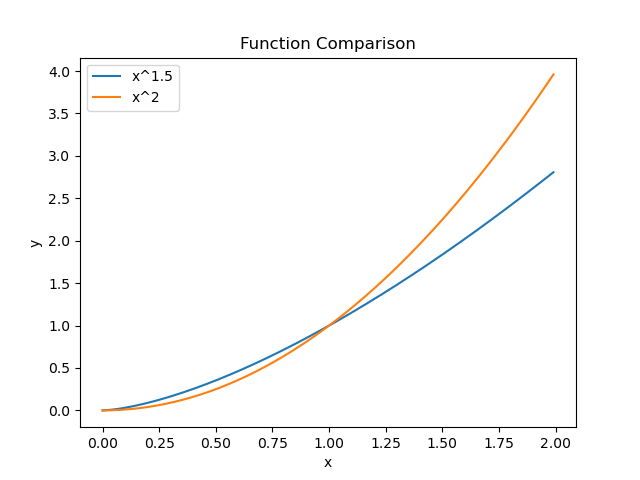
\includegraphics[width=0.7\textwidth]{../figures/Figure_1.png}
  \caption{Comparison of the functions $x^{1.5}$ and $x^2$ plotted using matplotlib.}
\end{figure}

% Figure 2
\begin{figure}[h!]
  \centering
  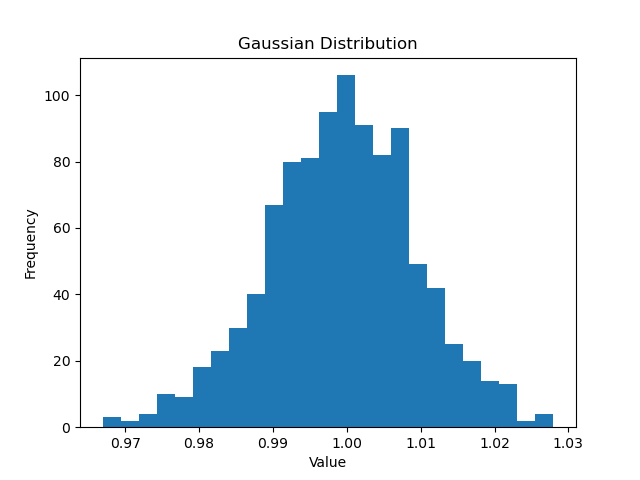
\includegraphics[width=0.7\textwidth]{../figures/Figure_2.png}
  \caption{Visualization of random points used to estimate $\pi$ using the Monte Carlo method.}
\end{figure}

% Figure 3
\begin{figure}[h!]
  \centering
  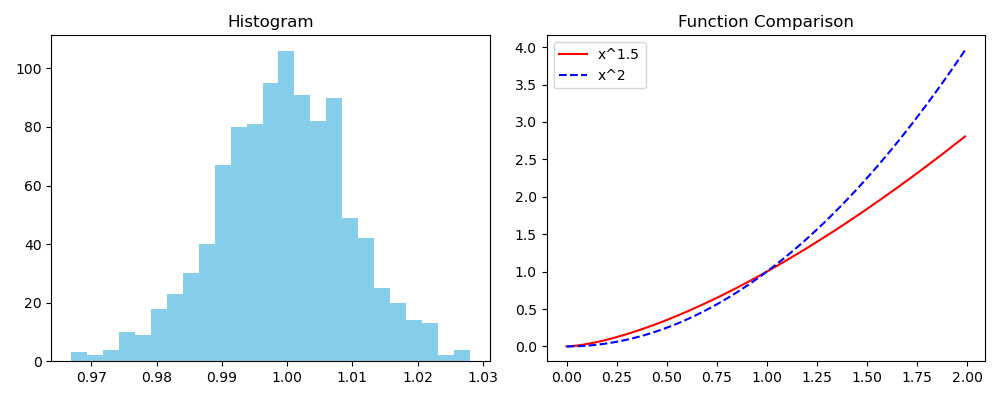
\includegraphics[width=0.7\textwidth]{../figures/Figure_3.png}
  \caption{Histogram of values drawn from a normal distribution, overlaid with the theoretical Gaussian curve.}
\end{figure}

% Figure 4
\begin{figure}[h!]
  \centering
  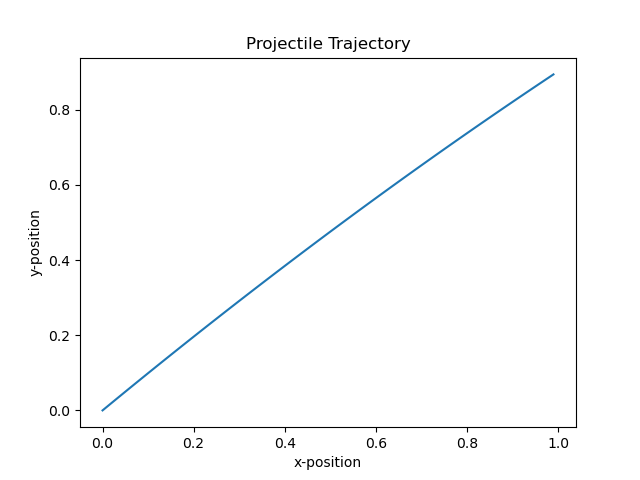
\includegraphics[width=0.7\textwidth]{../figures/Figure_4.png}
  \caption{Simulated trajectory of a projectile launched at a 45-degree angle.}
\end{figure}

% Figure 5
\begin{figure}[h!]
  \centering
  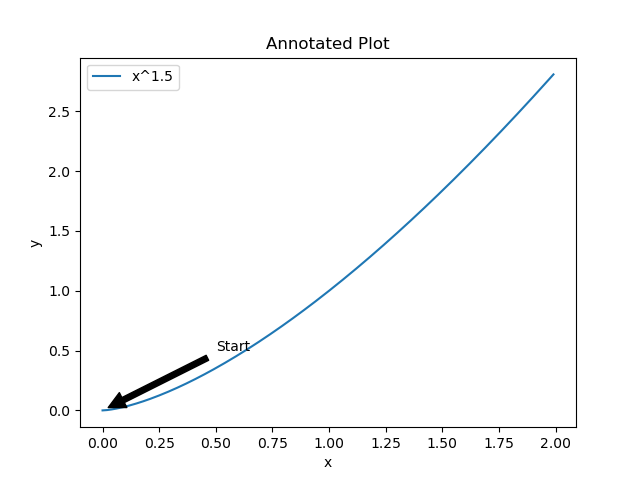
\includegraphics[width=0.7\textwidth]{../figures/Figure_5.png}
  \caption{Multi-panel plot showing both a histogram and a function comparison.}
\end{figure}

% Figure 6
\begin{figure}[h!]
  \centering
  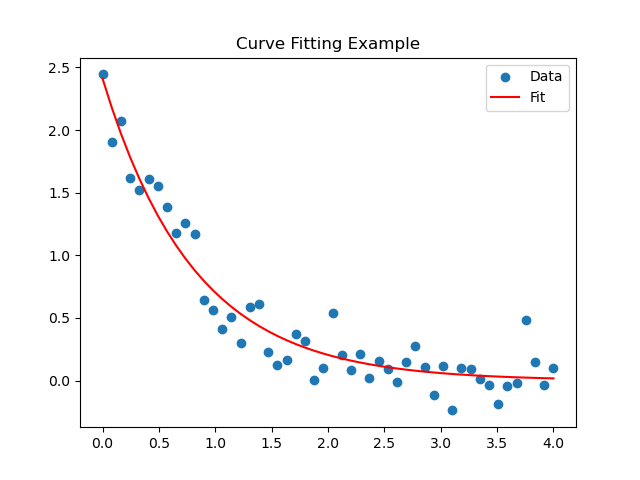
\includegraphics[width=0.7\textwidth]{../figures/Figure_6.png}
  \caption{Scatter plot of noisy data with an exponential decay fit.}
\end{figure}

% Figure 7
\begin{figure}[h!]
  \centering
  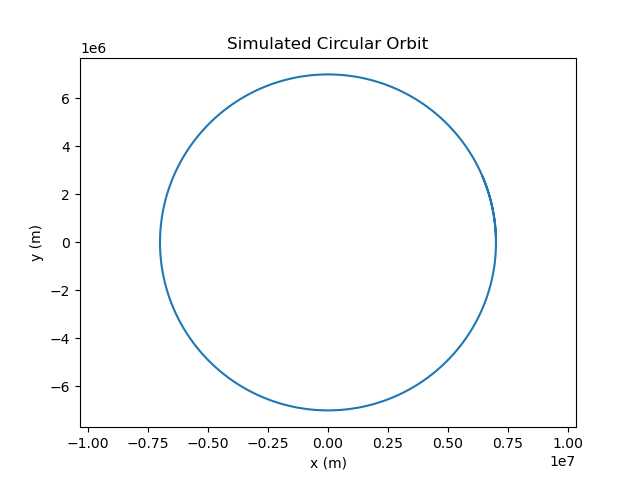
\includegraphics[width=0.7\textwidth]{../figures/Figure_7.png}
  \caption{Plot with error bars and scientific notation, illustrating uncertainty in measurements.}
\end{figure}

% Figure 8
\begin{figure}[h!]
  \centering
  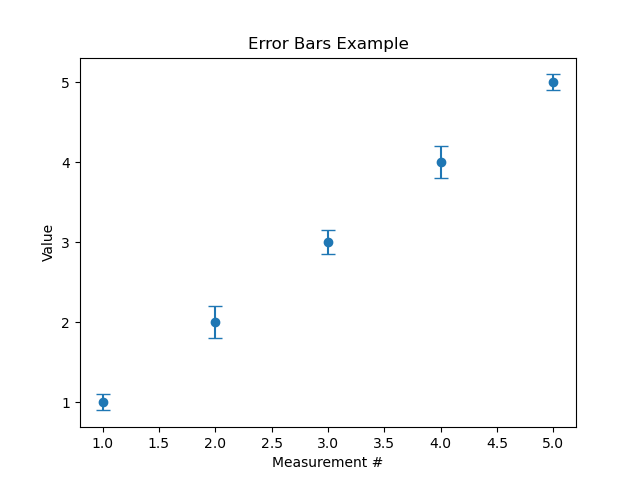
\includegraphics[width=0.7\textwidth]{../figures/Figure_8.png}
  \caption{Simulation of a circular orbit using basic physics and numpy.}
\end{figure}

% --- Data Files ---
\subsection*{Data Files}
\begin{itemize}
  \item \texttt{motion\_day8.csv}: CSV file containing time and position data for a simple motion experiment. Used for plotting and curve fitting in Day 8.
  \item \texttt{hello\_day5.txt}: Example text file created and read during Day 5 to demonstrate file I/O in Python.
  \item \texttt{data\_day5.txt}: Data file containing simulated values from a normal distribution, used for histogram plotting and statistical analysis.
\end{itemize}

\section*{Reflections and Insights}
Participating in Python4Physics 2025 was not only an academic experience but also a personal journey of growth. The daily structure, which combined lectures, hands-on coding, and collaborative projects, fostered a supportive and motivating environment. I found that learning alongside peers with diverse backgrounds encouraged me to approach problems from new perspectives and to communicate my ideas more clearly.

One of the most impactful aspects of the program was the opportunity to engage with guest lecturers who are active researchers in their fields. The session on computational astrophysics, for example, demonstrated how the concepts we practiced in class are applied to real-world scientific questions. This inspired me to consider how I might use computational tools in my own future research, whether in physics, engineering, or data science.

The capstone project in the final days of the program was a highlight. Working in a team, we tackled a complex problem that required integrating skills from across the curriculum: data analysis, simulation, visualization, and scientific communication. Presenting our results to the group was both challenging and rewarding, and the feedback we received helped me see the value of clear, reproducible code and effective storytelling with data.

Looking back, I am grateful for the challenges I encountered—especially those that initially seemed daunting, such as debugging code or interpreting unexpected results. These moments taught me resilience and the importance of seeking help and collaborating with others. I now feel equipped not only with technical skills but also with the confidence to tackle new problems and to continue learning independently.

\section*{Future Applications}
I plan to use the skills gained in Python4Physics in my future coursework and research. Whether analyzing experimental data, simulating physical systems, or visualizing results, I now feel confident in my ability to use Python as a powerful tool for scientific inquiry. I am also motivated to continue learning about advanced topics such as machine learning and computational modeling.

\section*{Conclusion}
Python4Physics 2025 has equipped me with practical skills in scientific programming and a deeper appreciation for computational physics. I am grateful for the opportunity to participate and look forward to applying these skills in future academic and research endeavors.

\vspace{1em}
\noindent\textbf{Thank you to the instructors, guest speakers, and fellow participants for making this a memorable and impactful experience.}

\end{document}
